\documentclass[a4paper,14pt]{extarticle}

\usepackage[utf8x]{inputenc}
\usepackage[T1,T2A]{fontenc}
\usepackage[russian]{babel}
\usepackage{hyperref}
\usepackage{indentfirst}
\usepackage{here}
\usepackage{array}
\usepackage{graphicx}
\usepackage{caption}
\usepackage{subcaption}
\usepackage{chngcntr}
\usepackage{amsmath}
\usepackage{amssymb}
\usepackage{pgfplots}
\usepackage{pgfplotstable}
\usepackage[left=2cm,right=2cm,top=2cm,bottom=2cm,bindingoffset=0cm]{geometry}
\usepackage{multicol}
\usepackage{askmaps}
\usepackage{titlesec}
\usepackage{listings}
\usepackage{color}
\usepackage{courier}

\definecolor{green}{rgb}{0,0.6,0}
\definecolor{gray}{rgb}{0.5,0.5,0.5}
\definecolor{purple}{rgb}{0.58,0,0.82}

\lstset{
	language=Verilog,
	backgroundcolor=\color{white},   
	basicstyle=\small\ttfamily,
	commentstyle=\color{green},
	keywordstyle=\color{blue},	
	numberstyle=\tiny\color{gray},
	stringstyle=\color{purple},
	breakatwhitespace=false,
	breaklines=true,
	captionpos=b,
	keepspaces=true,
	numbers=left,
	numbersep=5pt,
	showspaces=false,
	showstringspaces=false,
	showtabs=false,
	tabsize=4,
	frame=single,
	inputpath={../quartus/},
	literate={~} {$\sim$}{1}
}

\renewcommand{\le}{\ensuremath{\leqslant}}
\renewcommand{\leq}{\ensuremath{\leqslant}}
\renewcommand{\ge}{\ensuremath{\geqslant}}
\renewcommand{\geq}{\ensuremath{\geqslant}}
\renewcommand{\epsilon}{\ensuremath{\varepsilon}}
\renewcommand{\phi}{\ensuremath{\varphi}}
\renewcommand{\thefigure}{\arabic{figure}} 	
\renewcommand*\not[1]{\overline{#1}}

\titleformat*{\section}{\large\bfseries} 
\titleformat*{\subsection}{\normalsize\bfseries} 
\titleformat*{\subsubsection}{\normalsize\bfseries} 
\titleformat*{\paragraph}{\normalsize\bfseries} 
\titleformat*{\subparagraph}{\normalsize\bfseries} 

\counterwithin{figure}{section}
\counterwithin{equation}{section}
\counterwithin{table}{section}
\newcommand{\sign}[1][5cm]{\makebox[#1]{\hrulefill}}
\graphicspath{{../pics/}}
\captionsetup{justification=centering,margin=1cm}
\def\arraystretch{1.3}
\setlength\parindent{5ex}
\titlelabel{\thetitle.\quad}

\begin{document}

\begin{titlepage}
\begin{center}
	Санкт-Петербургский Политехнический Университет Петра Великого\\[0.3cm]
	Институт компьютерных наук и технологий \\[0.3cm]
	Кафедра компьютерных систем и программных технологий\\[4cm]
	
	\textbf{ОТЧЕТ}\\ 
	\textbf{по лабораторной работе}\\[0.5cm]
	\textbf{SystemVerilog №4}\\[0.1cm]
	Автоматизация проектирования\\ дискретных устройств\\[4.0cm]
\end{center}

\begin{flushright}
	\begin{minipage}{0.45\textwidth}
		\textbf{Работу выполнил студент}\\[3mm]
		группа 33501/4 \hspace*{9mm} Дьячков В.В.\\[5mm]
		\textbf{Преподаватель}\\[5mm]
		\sign[1.5cm] \hspace*{1mm} к.т.н., доц. Филиппов А.С. \\[5mm]
	\end{minipage}
\end{flushright}

\vfill

\begin{center}
	Санкт-Петербург\\
	\the\year
\end{center}
\end{titlepage}

\addtocounter{page}{1}
\counterwithin{lstlisting}{section}

\tableofcontents
\listoffigures
\lstlistoflistings
\listoftables
\newpage

\section{Задание}

\begin{itemize}
	\item Понимание причин возникновения сбоев, вызванных метастабильностью, и способов привязки асинхронных сигналов в Quartus Prime;
	\item Получение навыков анализа метастабильности с использованием TimeQuest Timing Analyzer.
\end{itemize}

\section{Выполнение работы}

\subsection{Компиляция и анализ проекта, задание временных требований}

В подготовленном заранее проекте \code{Metastabil}, приведенном на рис. \ref{fig:source}, не выполняются требования к времени установки.
\begin{figure}[H]
	\begin{center}
		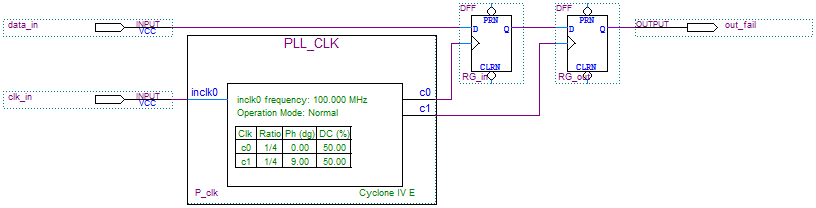
\includegraphics[width=\textwidth]{source}
		\caption{Исходный проект}
		\label{fig:source}
	\end{center}
\end{figure}

Зададим временные ограничения и режим анализа цепей синхронизации как \code{Forced If Asynchronous}. В листинге \ref{code:sdc} приведен SDC-файл.

\vspace{0.5cm}
\lstinputlisting[caption=SDC1.sdc, label=code:sdc]{SDC1.sdc}

\newpage

\subsection{Компиляция и анализ проекта с заданными временными требованиями и анализ результатов}

После компиляции можно заметить, что в проекте используется один заданный базовый тактовый сигнал с частотой 100 МГц. и два порожденных тактовых сигнала с заданными при настройке PLL частотами.
\begin{figure}[H]
	\begin{center}
		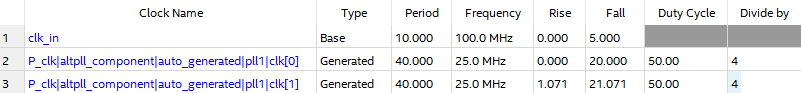
\includegraphics[width=\textwidth]{clocks_1}
		\caption{Тактовые сигналы}
		\label{fig:clocks_1}
	\end{center}
\end{figure}

В разделе Slow 1200mV 85C Model Setup Summary, приведенном на рис. \ref{fig:timing_1}, видно, что временные требования не выполняются. Однако для остальных моделей ошибок нет, следовательно может оцениваться метастабильность.

\begin{figure}[H]
	\begin{center}
		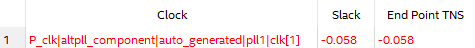
\includegraphics[scale=0.95]{timing_1}
		\caption{Slow 1200mV 85C Model Setup Summary}
		\label{fig:timing_1}
	\end{center}
\end{figure}

На рис. \ref{fig:paths_1} приведен отчет Report Exceptions в TimeQuest Timing Analyzer. Видно, что заданные пути исключены из анализа. 

\begin{figure}[H]
	\begin{center}
		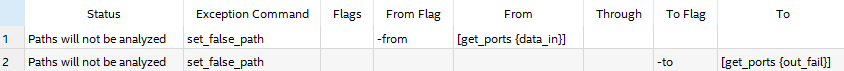
\includegraphics[width=\textwidth]{paths_1}
		\caption{Slow 1200mV 85C Model Setup Summary}
		\label{fig:paths_1}
	\end{center}
\end{figure}

\newpage

На рис. \ref{fig:waveform_1} изображена временная диаграмма для регистровой передачи \code{From Node RG_in To Node RG_out}. Тактовым сигналом, запускающим данные в данной регистровой передаче является сигнал с вывода \code{clk[0] PLL_CLK} (Launch Clock), а захватывающим - сигнал с вывода \code{clk[1] PLL_CLK} (Latch Clock). Временной интервал между ними соответствует фазовому сдвигу, заданному при настройке \code{PLL_CLK}.

\begin{figure}[H]
	\begin{center}
		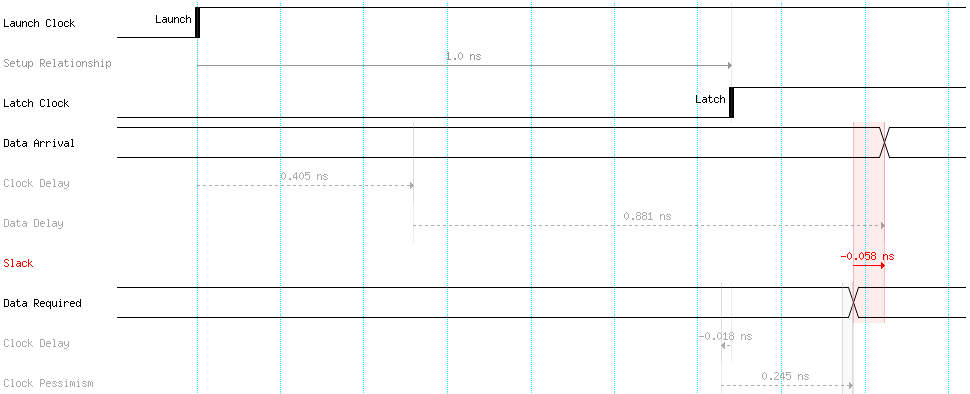
\includegraphics[width=\textwidth]{waveform_1}
		\caption{Slow 1200mV 85C Model Setup Summary}
		\label{fig:waveform_1}
	\end{center}
\end{figure}

Для обеспечения работоспособности цепи увеличим фазовый сдвиг на время отрицательного допуска Setup, равное 58 пс. Из отчета компиляции, приведенного на рис. \ref{fig:timing_2}, видно, что теперь временные требования выполнены. 

\begin{figure}[H]
	\begin{center}
		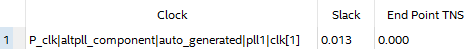
\includegraphics[scale=0.95]{timing_2}
		\caption{Slow 1200mV 85C Model Setup Summary}
		\label{fig:timing_2}
	\end{center}
\end{figure}

Полученный проект не содержит временных ошибок и для него может проводиться анализ метастабильности для всех моделей задержек. Установлен минимальный положительный допуск Setup, для которого интенсивность сбоев, вызванных метастабильностью, будет максимальной.

\newpage

\subsection{Анализ интенсивности сбоев, вызванных метастабильностью}

На рис. \ref{fig:assignments_1} приведена заданная активность переключений в Assignment Editor, равная 20 МГц.

\begin{figure}[H]
	\begin{center}
		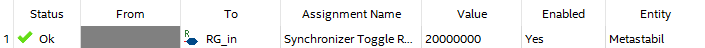
\includegraphics[scale=0.95]{assignments_1}
		\caption{Активность переключений в Assignment Editor}
		\label{fig:assignments_1}
	\end{center}
\end{figure}

На рис. \ref{fig:timing_3} приведен Metastability Report для модели Slow 1200mV 85C Model Setup. Из отчета видно, что частота переключений Data Toggle Rate, используемая для вычисления Mean Time Before Faille (MTBF), соответствует заданной.

\begin{figure}[H]
	\begin{center}
		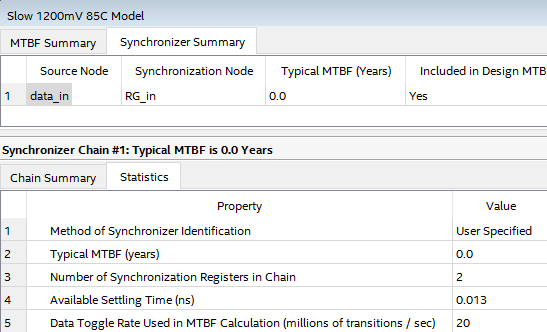
\includegraphics[scale=0.95]{timing_3}
		\caption{Metastability Report для Slow 1200mV 85C Model}
		\label{fig:timing_3}
	\end{center}
\end{figure}

В таблице \ref{tab:research} приведены результаты исследования для разных моделей и значений сдвига фазы \code{clk[1]}.

\begin{table}[H]
	\centering
	\small
	\caption{Исследование метастабильности}
	\label{tab:research}
	\begin{tabular}{|c|P{0.17\linewidth}|P{0.1\linewidth}|P{0.11\linewidth}|P{0.1\linewidth}|P{0.11\linewidth}|P{0.1\linewidth}|P{0.11\linewidth}|}
		\hline
		\multirow{2}{*}{\makecell{\\ \\ №}} & \multirow{2}{*}{\makecell{\\ Сдвиг фазы / \\ Output slack, нс}} & \multicolumn{2}{l|}{\makecell{\centering Slow 85C}} & \multicolumn{2}{l|}{\makecell{Slow 0C}} & \multicolumn{2}{l|}{\makecell{\centering Fast 0C}} \\ \cline{3-8} 
		&  & Available Setting Time, нс & Typical MTBF, лет & Available Setting Time, нс & Typical MTBF, лет & Available Setting Time, нс & Typical MTBF, лет \\
		\hline
		1 & 1.058 & 0.013 & 0 & 0.121 & 0 & 0.602 & 2.63e-06 \\
		\hline
		2 & 1.258 & 0.192 & 0 & 0.300 & 0 & 0.781 & 1.85e-04 \\
		\hline
		3 & 1.458 & 0.400 & 0 & 0.508 & 2.82e-07 & 0.989 & 2.58e-02 \\
		\hline
		4 & 1.658 & 0.608 & 3.03e-06 & 0.716 & 3.94e-05 & 1.197 & 3.61 \\
		\hline
		5 & 1.858 & 0.817 & 4.34e-04 & 0.925 & 5.65e-3 & 1.406 & 517 \\
		\hline
		6 & 2.058 & 0.987 & 2.46e-02 & 1.095 & 0.32 & 1.576 & 2.93e+04 \\
		\hline
		7 & 2.258 & 1.192 & 3.21 & 1.300 & 41.7 & 1.781 & 3.82e+06 \\
		\hline
		8 & 2.458 & 1.442 & 1.22e+03 & 1.550 & 1.58e+04 & 2.031 & 1e+09 \\
		\hline
		9 & 2.658 & 1.650 & 1.70e+05 & 1.758 & 2.21e+06 & 2.239 & 1e+09 \\
		\hline
		10 & 2.858 & 1.799 & 5.86e+06 & 1.907 & 7.62e+07 & 2.388 & 1e+09 \\
		\hline
		11 & 3.058 & 1.997 & 6.46e+08 & 2.105 & 1e+09 & 2.586 & 1e+09 \\
		\hline
		12 & 3.258 & 2.192 & 1e+09 & 2.300 & 1e+09 & 2.781 & 1e+09 \\
		\hline
	\end{tabular}
\end{table}

\noindent Подключим вход синхронизации триггера \code{RG_out} к выходу \code{c0 PLL_CLK}:
\begin{itemize}
	\item Available Setting Time = 39.036 нс
	\item Typical MTBF = 1e+09 лет
\end{itemize}

\noindent Установим тактовую частоту на выходе \code{c0 PLL_CLK} равной 400 МГц:
\begin{itemize}
	\item Available Setting Time = 39.036 нс
	\item Typical MTBF = 1e+09 лет
\end{itemize}

\noindent Установим цепь синхронной привязки сигналов с тремя триггерами:
\begin{itemize}
	\item Available Setting Time = 78.074 нс
	\item Typical MTBF = 1e+09 лет
\end{itemize}

%\section{Контрольные вопросы}
%
%\begin{itemize}
%	\item Что такое MTBF?
%	
%	Mean Time Between Failures – среднее время между сбоями.
%	
%	\item Соответствуют ли полученные результаты экспериментальных исследований увеличению значения MTBF в 10.8 раз при увеличении Available Setting Time на 100 пс?
%	
%	Из 9-10 строк таблицы можно найти, что MTBF увеличилось в 34 раз при изменении Available Setting Time на 149 пс, что соответствует увеличению в 22 раза на 100 пс.
%	
%	\item Назовите причины, по которым результаты, полученные на компьютерной модели (Quartus II) могут не соответствовать результатам на физической модели.
%	
%	Наличие посторонних помех, особенности проводников (сопротивление, длина и т.д.), коррозия металла, внешние условия, при которых используется устройство, «старение» электронных компонентов, то есть их износ.
%	
%	\item Почему микросхема с большим быстродействием обеспечивает меньшую интенсивность сбоев при прочих равных условиях?
%	
%	Большее быстродействие обеспечивает более быструю обработку ситуации, которая может привести к сбою, следовательно, при большем быстродействии сбоя может не произойти.
%	
%	\item Почему наличие логики между триггерами принимающего данные тактового домена увеличивает MTBF?
%	
%	Отсутствие логики создает слишком малую задержку между триггерами. Если они синхронизируются разными тактовыми доменами, малая задержка может привести к сбою. 
%	
%	\item Как наличие логики между триггерами принимающего данные домена имитируется в выполняемой работе?
%	
%	С помощью сдвига фазы тактовых частот на 1 нс.
%\end{itemize}

\section{Выводы}

В работе выполнены типовые задания временных требований к синхронному проекту. Для анализа метастабильности обеспечена работоспособность проекта с заданными частотами, исключены из временного анализа пути, для которых определялась метастабильность, выполнены настройки компилятора, обеспечивающие анализ взаимодействия асинхронных тактовых доменов. Оценено влияние допуска Setup и количества синхронизирующих триггеров на интенсивность сбоев.

\end{document}